% Name: Free-body diagram
% Description: A block on a level floor with its weight, the normal force, a pull, and friction, each drawn from its center.
% Tags: free-body diagram, forces, Newton's laws, friction

\usetikzlibrary{arrows.meta, patterns}

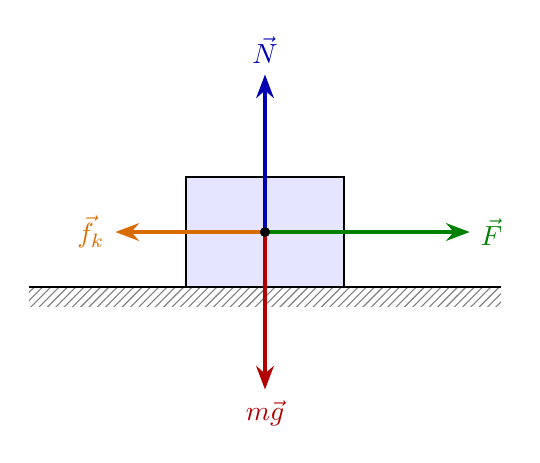
\begin{tikzpicture}[>={Stealth[length=3mm]}, force/.style={->, very thick}]
  \fill[pattern=north east lines, pattern color=gray] (-3,-0.25) rectangle (3,0);
  \draw[thick] (-3,0) -- (3,0);
  \draw[thick, fill=blue!10] (-1,0) rectangle (1,1.4);
  \coordinate (c) at (0,0.7);
  \draw[force, red!70!black] (c) -- (0,-1.3) node[below] {$m\vec{g}$};
  \draw[force, blue!70!black] (c) -- (0,2.7) node[above] {$\vec{N}$};
  \draw[force, green!50!black] (c) -- (2.6,0.7) node[right] {$\vec{F}$};
  \draw[force, orange!85!black] (c) -- (-1.9,0.7) node[left] {$\vec{f}_k$};
  \fill (c) circle (1.8pt);
\end{tikzpicture}
